\section{Robotics Framework for Reliable Trajectory Execution}\label{sec:architecture}

\subsection{Robotics Architecture}

In this section the main components of our robotics framework for
reliable trajectory estimation will be described. The HRP-2 robot
embeds two computers. One is dedicated to motor control and the other
one to vision processing. Fig.~\ref{fig:framework_overview}
illustrates the complete robotics distributed infrastructure used in
this experiment. It relies heavily on both OpenHRP and ROS to
integration the different modules altogether.
%
\begin{figure}[ht!]
  \begin{center}
    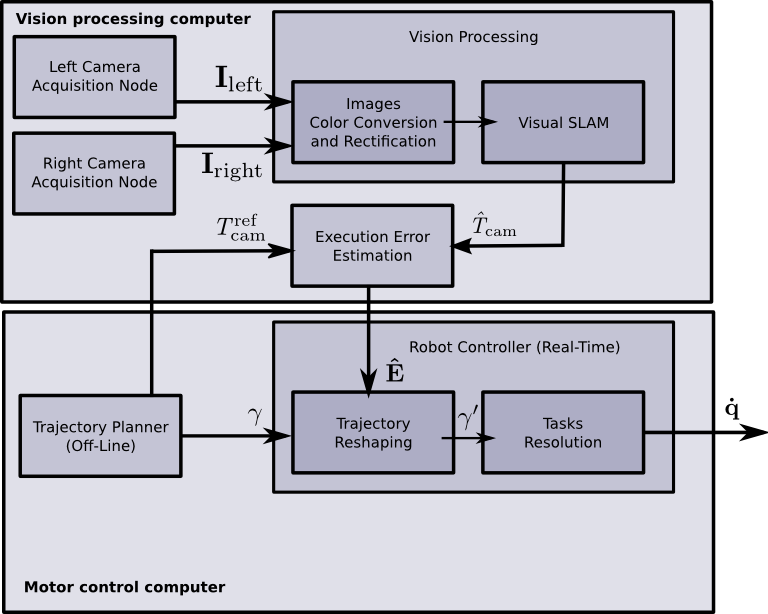
\includegraphics[width=\linewidth]{images/rss_framework.png}
  \end{center}
  \caption{Complete robotics framework overview. Let
    $\mathbf{I}_{\text{left}}$, $\mathbf{I}_{\text{right}}$ be
    respectively the left and right camera
    images. $\mathit{T}_{\text{cam}}$, $\mathit{\hat{T}}_{\text{cam}}$
    respectively the planned and estimated camera
    position. $\mathbf{\gamma}$ the concatenation of the left ankle,
    right ankle, upper body and center of mass
    trajectories. $\mathbf{\gamma'}$ the trajectories reshaped by
    taking into account execution
    errors.\label{fig:framework_overview}}
\end{figure}
% The control is based on a task based
controller~\cite{Mansard09icar}. A task is a function which associates
\mbox{$\mathbf{q} \in \mathcal{C}$} the robot configuration to
\mbox{$e(\mathbf{q}) \in \mathbb{R}$} an error. The controller embeds
a solver which is able to generate a control law which minimizes the
error for a given stack of tasks.

\begin{enumerate}
\item Using a given stack of tasks, this controller computes the joint
  velocities $\mathbf{\dot{q}}$ which realizes the tasks. Our stack of
  tasks ensures that the left ankle, right ankle, center of mass and
  upper level posture reference positions are followed. The reference
  trajectories are computed off-line by the planner described in
  \cite{Dalibard11humanoids}.
\item The reference trajectories can be post-processed by the
  controller to reshape them on the fly. The controller has been
  extended to incorporate a module which can, given an execution error
  estimation, cancel them automatically by changing the future robot
  trajectory.
\item This estimation of the execution error is computed on the
  computer dedicated to vision. By comparing the planned left ankle
  trajectory and the estimated one, it is possible to compute an
  estimation of the execution error.
\item The planned left ankle position is computed using both the
  camera position and the relative transformation from the camera to
  the left ankle. This transformation can be deduced from the robot
  configuration and its model using forward kinematics.
\end{enumerate}

\subsection{Closed-loop tracking}

Closed-loop trajectory tracking consists in following a precomputed
trajectory while compensating for execution errors. Systems are often
composed of four components:
\begin{enumerate}
\item a trajectory generator component,
\item a localization component providing an estimation of the robot
  position,
\item an error estimation component computing the error between the
  planned position and the localization of the robot,
\item and a component reshaping the planned trajectory to compensate
  for the above error.
\end{enumerate}


The trajectory generator provides two reference data: the footstep
sequence, a set of footsteps $S_i$ such as \mbox{$0 \leq i \leq
  n^{\text{step}}$} and a whole-body trajectory \mbox{$\gamma(t \in
  [t_{\text{min}}, t_{\text{max}}]) \in \mathcal{C}$}. One advantage
of the proposed control scheme is to alter the future footstep
positions to avoid singularities. Given a known perturbation of the
footstep sequence, it is then possible to deduce the correction that
should be applied to the feet and center of mass trajectories. Once
those trajectories are computed, inverse geometry can be used to
regenerate the joints trajectories.


One iteration of the control loop is described by
Algorithm~\ref{fig:control_loop} and can be summarized as:
\begin{enumerate}
\item estimate the robot position,
\item compute the position error \mbox{$\delta \mathbf{x}$},
\item filter the error to avoid perturbing too much the initial
  trajectory and to absorb localization noise,
\item recompute the next steps positions to compensate execution
  errors and make sure the feet will land on the planned position,
\item check if the recomputed next step is feasible,
\item regenerate smooth trajectories for the feet, center of mass and
  ZMP.
\item regenerate the joints trajectories. This step is denoted by
  \mbox{$\gamma \bigoplus \delta \gamma$} in the algorithm. The
  \mbox{$\gamma \bigoplus \delta \gamma$} operation returns $\gamma$
  altered by the rigid transformation \mbox{$\delta \gamma$}. $\delta
  \gamma$ is the perturbation applied to the whole-body trajectory and
  is not directly computed as the inverse geometry is directly applied
  on the updated body positions.
\end{enumerate}


\begin{algorithm}
  \begin{algorithmic}
    \REQUIRE {$\gamma$, $t_{\text{current}}, t_{\text{next\_correction}}$}
    \ENSURE {$\gamma$, $t_{\text{current}}, t_{\text{next\_correction}}$}
    \IF {$\gamma(t_{\text{current}})$ is double support \AND
      $t_{\text{current}} \geq t_{\text{next\_correction}}$}
    \STATE estimate robot position $\mathbf{\hat{x}}$
    \STATE compute robot position error $\delta \mathbf{x}$
    \STATE compute offset $\delta \gamma$ absorbing the execution
    error $\delta \mathbf{x}$
    \IF {the perturbation $\delta \gamma$ can be applied}
    \STATE $\forall t \in [t_{\text{current}}, t_{\text{max}}],
    \gamma(t) \leftarrow \gamma(t) \bigoplus \delta \gamma(t)$
    \STATE $t_{\text{next\_correction}} \leftarrow t_{\text{current}} + 2 T_{\text{step}}$
    \ENDIF
    \ENDIF
    \STATE $\mathbf{q} \leftarrow \gamma(t_{\text{current}})$
    \STATE $t_{\text{current}} \leftarrow t_{\text{current}} + \Delta t$
  \end{algorithmic}
  \caption{Control loop at time $t_{\text{current}}$ achieving a
    closed-loop following of trajectory $\gamma$ (next correction will
    be applied at
    $t_{\text{next\_correction}}$). \label{fig:control_loop}}
\end{algorithm}


First, the robot position $\hat{\mathbf{x}}$ is perceived. The
localization system will not be detailed in this paper, see
\cite{08ijhr.stasse, 06humanoids.thompson} for instance for more
details. Although common limitations of these systems are taken into
account. The precision of the robot estimation does not decrease over
time, but can vary during the execution. This produces a noise which
may perturb the control scheme. The localization system can also fail
to provide an estimation or even sometimes provide aberrant values.

Secondly, an error $\mathbf{\delta \mathbf{x}}$ is computed by
comparing the planned and estimated position of the tracked reference
body. A threshold is applied to this value to bound the applied
corrections. In practice, it also filters out outliers and the noise
that the localization system may introduce in the system.

Then, the relative position of the next footstep w.r.t. to the current
one is changed to compensate the perceived
error. Fig.~\ref{fig:footstepreplan} illustrates this process.


From this point, smooth trajectories can be regenerated for feet and
center of mass. To ensure smoothness, the trajectory correction is
progressively applied during the next two steps. To finish, joint
values are recomputed using these new reference trajectories.



Additionally, a test is added to check that a correction can be
computed for the current time $t_{\text{current}}$. A correction can
be applied if no correction is being applied,
i.e.\ \mbox{$t_{\text{current}} \geq t_{\text{next\_correction}}$} and if the
robot is in the double support phase. Indeed starting a correction in
the middle of a step would be dangerous and starting a correction
while another correction is being applied would lead to erroneous
results.


Previous works such as \cite{04humanoids.harada, 07icra.morisawa} aim
at allowing sudden changes in the robot trajectory. The proposed
control scheme is different and aim at following as closely as
possible a preplanned trajectory.


\paragraph{Estimation of the position error}

We make the assumption that an external system provides
\mbox{$\hat{\mathbf{x}} \in \text{SE}(2)$}, an estimation of the
current robot position.

If $\mathbf{x} \in \text{SE}(2)$ is the robot planned position and
$\hat{\mathbf{x}} \in \text{SE}(2)$ the robot localization, the
position error is defined by:

\begin{equation} \label{eq:errorpos}
  \mathbf{\delta x} = \mathbf{x} . \hat{\mathbf{x}}^{-1}
\end{equation}

In Eq. (\ref{eq:errorpos}), $\mathbf{\delta x}(t)$ can be
interpreted as the planned robot position with respect to the current
robot position at time $t$. By consequence, at the beginning of the
trajectory $t_{\text{min}}$, the error is always equal to zero:

\begin{equation} \label{eq:errorpos_prop}
  \delta \mathbf{x}(t_{\text{min}}) = 0
\end{equation}

\paragraph{Footstep sequence modification}


Given a position error of the waist, it is possible to alter the
remaining steps in the footstep sequence to absorb this offset.

The purpose of this step is to take into consideration that the
previous step has not been executed correctly, leading to a different
relative position than the one which has been initially planned. To
cancel the error, the next footsteps positions will be modified
so that the robot will step in the planned locations.


The footstep positions are \mbox{$S \in
  \text{SE}(2)^{n^\text{step}}$}. Let consider $\mathbf{\delta {x}}$,
the current position error, \mbox{$S^{\text{future}} \subset S$} the
steps which have not been played yet. The footstep positions will be
changed according to the following computation:

\begin{equation} \label{eq:footstepmodif}
  \forall s \in S^{\text{future}}, s \gets \mathbf{\delta {x}} . s
\end{equation}


\paragraph{Whole-body trajectories modification}

A new placement of the next feet has been computed. It is now necessary
to modify the two feet and the center of mass trajectories
synchronously to reach the corrected foot prints.

The correction is computed by considering the simplified model
introduced in section \ref{problem}. Hence, no hypothesis is done on
the strategy used to plan the reference trajectories. One interest of
this approach is to totally dissociate the planning and correction
algorithms. To compute a small perturbation the simplified model is
sufficient. It allows extremely reactive correction without
compromising the overall trajectory quality.


The linearized inverse pendulum model allows the computation of the
center of mass trajectory $\mathbf{c}(t)$ given a ZMP trajectory
$\mathbf{z}(t)$ by solving Eq.~(\ref{eq:zmp1}). Considering $\mathbf{r}$ a
polynomial depending only of $\mathbf{z}$, $(V_x, V_y, W_x, W_y)$ free
parameters used to constrain the initial position and velocity of the
center of mass, a general following form of a polynomial center of
mass trajectory is:

\begin{equation} \label{eq:zmpsol}
  \mathbf{c}(t) = \cosh(\sqrt{\frac{g}{z_c}}.t) . \mathbf{V} + \sinh(\sqrt{\frac{g}{z_c}}.t) . \mathbf{W} + \mathbf{r}(t)
\end{equation}

Given the formulation in Eq.~(\ref{eq:zmpsol}), it is possible to
continuously modify the center of mass trajectory to make it follow
\mbox{$\bar{\mathbf{z}}(t)$} the corrected trajectory. This new
trajectory can be expressed as the sum of two polynomials:

\begin{equation} \label{eq:zmpsolcor}
  \bar{\mathbf{c}}(t) = \cosh(\sqrt{\frac{g}{z_c}}.t) . \mathbf{V} +
  \sinh(\sqrt{\frac{g}{z_c}}.t) . \mathbf{W} + \mathbf{r}(t) + \mathbf{\Delta}(t)
\end{equation}

To apply smoothly the correction from $t_1$ to $t_2$, several
constraints expressed in Eq.~\ref{eq:cst} have to be respected.
$\delta \mathbf{x}_x$ and $\delta \mathbf{x}_y$ are respectively the
$x$ and $y$ components of the 2d rigid transformation $\delta
\mathbf{x}$.

\begin{equation}
\begin{aligned}
  \mathbf{\Delta}(t_1) &= 0\\
  \mathbf{\Delta}(t_2) &= \left(
  \begin{array}{c}
    \delta \mathbf{x}_x \\
    \delta \mathbf{x}_y
  \end{array}
  \right)\\
  \frac{\partial \mathbf{\Delta}}{\partial t}(t_1) = \frac{\partial
    \mathbf{\Delta}}{\partial t}(t_2) &= 0
\end{aligned}
\label{eq:cst}
\end{equation}

These four constraints determine the polynomial four parameters
leading to the curve illustrated by Fig.~\ref{fig:transition}.


This reshapes the center of mass trajectory by taking advantage of the
linear formulation of the simplified model. Additionally, the feet
trajectories are modified to reach the corrected positions at the end
of the step. The smooth correction is also obtained by using a third
degree polynomial with similar constraints: initial position remains
as before, the goal position must fit the corrected position and the
velocity of the correction is equal to zero at the beginning and the
end of the transition. Fig.~\ref{fig:traj} compares resulting
trajectories before and after the correction.


These three corrections must be executed in the correct order: as
stated before a correction is computed during a double support phase
and applied during the next two steps. We will make the assumption,
without any loss of generality, that the next flying foot is the left
one. In that case the correction of the left foot is progressively
applied during the single support phase. During the ZMP shift of this
step, the center of mass correction is also applied. Then, during the
next step, the correction of the right foot is applied. The timeline
of the correction is illustrated by Fig.~\ref{fig:traj}.


\PFA{This section can be dedicated to the control and planning framework}

%%% Local Variables:
%%% ispell-local-dictionary: "american"
%%% LocalWords:  odometry HRP
%%% End:
